% La SVD: leer la forma de las curvas de nivel
% Números y figuras PNG: apunte/scripts/cap07_svd.py (uv run python apunte/scripts/cap07_svd.py)
\chapter{La SVD: leer la forma de las curvas de nivel}\label{cap:svd}

\section{La idea}

Este capítulo parte de una observación de campo: muchas magnitudes que medimos no se reparten
igual en todas las direcciones. Una nube de lecturas repetidas se estira más en un sentido que
en otro, y una matriz estira más unas direcciones que otras. La herramienta que mide esos
estiramientos, dirección por dirección, es la descomposición en valores singulares (SVD, por
sus siglas en inglés). La presentamos como lo que es geométricamente: una manera de
\emph{leer} la forma de ciertas curvas de nivel.

\paragraph{Convenciones del capítulo.} Puntos y vectores en minúscula cursiva (\(x\), \(v\),
\(u\)), escritos en el texto como \((x_1,x_2)\) y en las cuentas como columnas; matrices en
mayúscula itálica (\(A\), \(U\), \(V\), \(\Sigma\), \(C\)); \(A^T\) es la transpuesta,
\(\det A\) el determinante, \(I\) la identidad y \(\|x\|\) la norma euclídea. Los valores
singulares se escriben \(\sigma_1\ge\sigma_2\ge\dots\ge0\); los autovalores, \(\lambda\); los
vectores singulares derechos (de la entrada), \(v_i\), y los izquierdos (de la salida),
\(u_i\). La letra \(Q\) queda reservada para la forma cuadrática \(Q(x)=x^TA^TAx=\|Ax\|^2\) y
\(N\) para la cantidad de puntos de una nube.

\subsection{Una pregunta de campo: el error que tiene dirección}

Supongamos que un receptor GNSS registra \(N=200\) posiciones de un mismo punto fijo y que
anotamos, en metros, cuánto se aparta cada posición (este, norte) del promedio. Los datos de
la figura~\ref{fig:svd-nube} son \emph{sintéticos}: los generó el script del capítulo con
semilla fija, imponiendo una dispersión mayor en una dirección que en la perpendicular, como
ocurre cuando la geometría de los satélites visibles determina mejor la posición en un
sentido que en otro. La nube no es redonda: se alarga en una dirección y se adelgaza en la
perpendicular. Las dos preguntas naturales son \emph{hacia dónde} se alarga y \emph{cuánto}.

\begin{figure}[htbp]
\centering
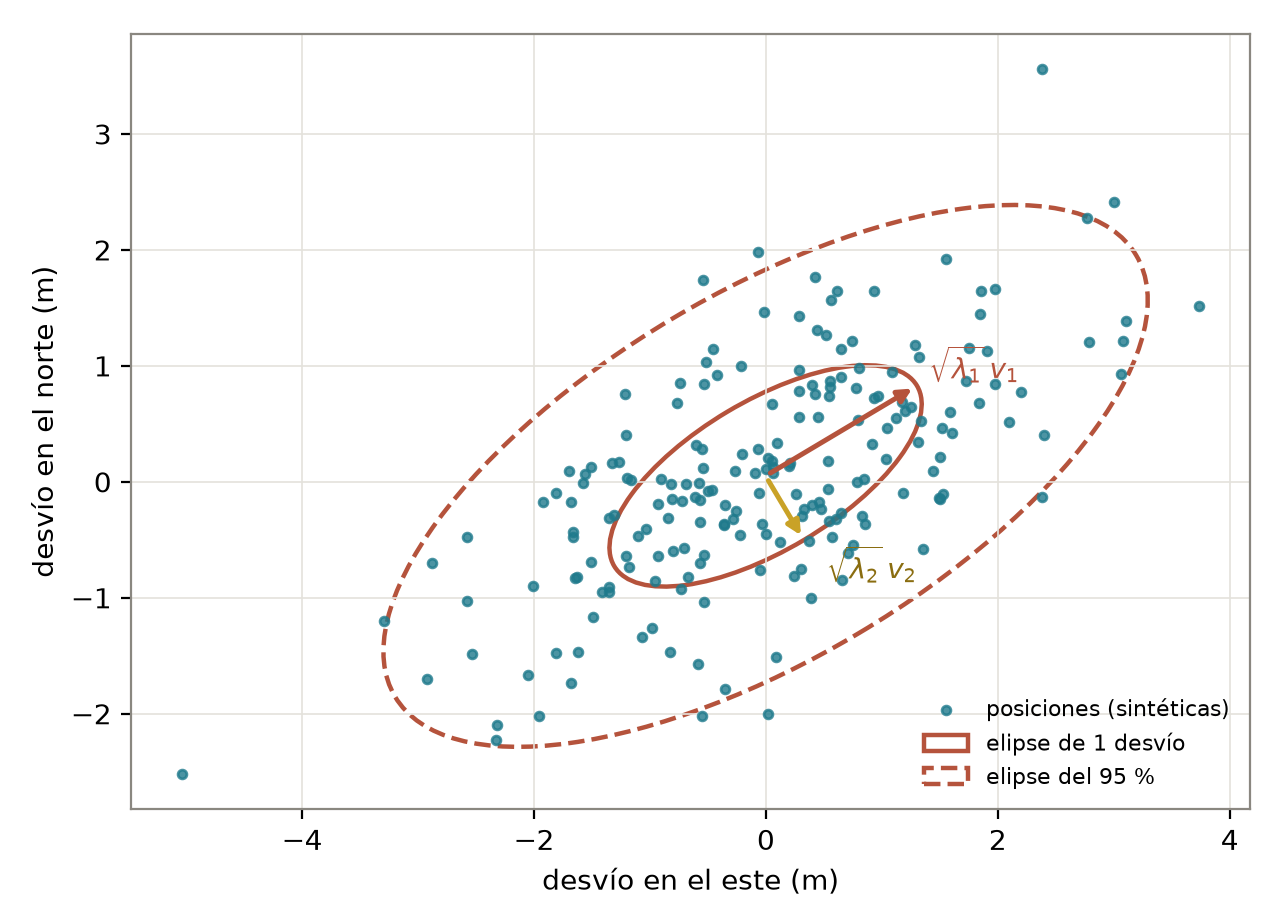
\includegraphics[width=.8\linewidth]{figuras/svd/svd_nube.png}
\caption{Doscientas posiciones GNSS sintéticas de un mismo punto, como desvíos en metros
respecto del promedio. La elipse de un desvío tiene sus ejes en las direcciones \(v_1\),
\(v_2\) y semiejes \(\sqrt{\lambda_1}\approx1{,}52\) m y \(\sqrt{\lambda_2}\approx0{,}64\) m;
la de trazos es la elipse del \(95\)\,\% (ejemplo~\ref{ej:svd-elipse-error}). Generada con \texttt{apunte/scripts/cap07\_svd.py}.}
\label{fig:svd-nube}
\end{figure}

La respuesta es una elipse: la \emph{elipse de error}. En el
ejemplo~\ref{ej:svd-elipse-error} la calculamos: su eje mayor está orientado
\(59{,}2^\circ\) respecto del norte y el \(95\)\,\% de las posiciones cae dentro de una
elipse de semiejes \(3{,}72\) m y \(1{,}58\) m. Para llegar ahí necesitamos dos piezas: qué funciones tienen
elipses como curvas de nivel y cómo se leen los ejes de esas elipses.

\subsection{Formas cuadráticas y sus curvas de nivel}

En el capítulo~\ref{cap:formas-lineales} vimos que una forma lineal, por ejemplo
\(\varphi(x)=2x_1+3x_2\), tiene como curvas de nivel una familia de \emph{rectas paralelas}
equiespaciadas: \(2x_1+3x_2=c\). El paso siguiente en complejidad es una función de grado
dos.

\begin{definicion}[Forma cuadrática]
Una \emph{forma cuadrática} en \(\R^n\) es una función \(x\mapsto x^TMx\), donde \(M\) es una
matriz simétrica de \(n\times n\). En este capítulo trabajamos con el caso
\[
  Q(x)=x^TA^TAx=\|Ax\|^2 ,
\]
donde \(A\) es una matriz de \(m\times n\) cualquiera y \(M=A^TA\) es automáticamente
simétrica. Su \emph{curva de nivel} \(c\) es el conjunto de los \(x\) con \(Q(x)=c\).
\end{definicion}

\(Q(x)\) mide el cuadrado del largo de la imagen de \(x\). Para la matriz que usaremos de
ejemplo en todo el capítulo,
\[
  A=\begin{pmatrix}3&0\\4&5\end{pmatrix},\qquad
  Q(x)=(3x_1)^2+(4x_1+5x_2)^2=25x_1^2+40x_1x_2+25x_2^2 .
\]
El término cruzado \(40x_1x_2\) impide leer la forma de las curvas \(Q=c\) a simple vista.
Pero si \(A\) es invertible, \(Q(x)=0\) sólo en el origen, \(Q\) crece como el cuadrado de la
distancia y es la misma en \(x\) y en \(-x\): sus curvas de nivel son curvas cerradas y
simétricas alrededor del origen, y vamos a ver que son \emph{elipses} concéntricas, todas de
la misma forma, con los mismos ejes (figura~\ref{fig:svd-curvas-nivel}).

\begin{figure}[htbp]
\centering
\begin{tikzpicture}[scale=1.5]
  % panel izquierdo: forma lineal, rectas paralelas
  \begin{scope}
    \clip (-1.5,-1.5) rectangle (1.5,1.5);
    \foreach \c in {-4,-3,...,4}
      \draw[teal,line width=.8pt] (-1.5,{(\c+3)/3}) -- (1.5,{(\c-3)/3});
  \end{scope}
  \draw[axisline] (-1.5,0)--(1.5,0); \draw[axisline] (0,-1.5)--(0,1.5);
  \draw[rust,line width=1pt,-{Latex[length=2mm]}] (0,0)--(.4,.6) node[above right,font=\small,labelback] {\((2,3)\)};
  \node[text=muted,font=\small,align=center] at (0,-1.9) {forma lineal \(\varphi(x)=2x_1+3x_2\):\\ rectas paralelas};
  % panel derecho: forma cuadrática, elipses
  \begin{scope}[xshift=4cm]
    \draw[axisline] (-1.5,0)--(1.5,0); \draw[axisline] (0,-1.5)--(0,1.5);
    \draw[auxline] (-1.06,-1.06)--(1.06,1.06) node[above right,font=\small,text=rust,labelback] {eje de \(v_1\)};
    \draw[auxline] (-1.06,1.06)--(1.06,-1.06) node[below right,font=\small,text=tealdark,labelback] {eje de \(v_2\)};
    \foreach \r in {1,2,3}
      \draw[mainline,rotate=45] (0,0) ellipse ({0.1491*\r} and {0.4472*\r});
    \node[font=\scriptsize,labelback] at (-.18,.62) {\(1\)};
    \node[font=\scriptsize,labelback] at (-.48,.98) {\(2\)};
    \node[font=\scriptsize,labelback] at (-.78,1.32) {\(3\)};
    \node[text=muted,font=\small,align=center] at (0,-1.9) {forma cuadrática \(\|Ax\|=1,2,3\):\\ elipses concéntricas};
  \end{scope}
\end{tikzpicture}
\caption{Curvas de nivel de una forma lineal (izquierda) y de \(Q(x)=\|Ax\|^2\) con
\(A=\left(\begin{smallmatrix}3&0\\4&5\end{smallmatrix}\right)\) (derecha), para
\(\|Ax\|=1,2,3\). Las elipses tienen sus ejes sobre las direcciones singulares \(v_1\)
(eje corto) y \(v_2\) (eje largo); el semieje corto de \(\|Ax\|=1\) mide
\(1/\sigma_1\approx0{,}149\) y el largo \(1/\sigma_2\approx0{,}447\).}
\label{fig:svd-curvas-nivel}
\end{figure}

\begin{idea}[Grado uno da rectas paralelas; grado dos da elipses concéntricas]
Las curvas de nivel de una forma lineal son rectas paralelas: la función crece igual en toda
una dirección y no distingue ningún punto. Las de una forma cuadrática \(\|Ax\|^2\) con \(A\)
invertible son elipses concéntricas: la función tiene un mínimo en el origen y crece más
rápido en unas direcciones que en otras. La pregunta del capítulo es cómo leer esas elipses.
\end{idea}

\subsection{La SVD como lectura de esas elipses}\label{sec:svd-idea}

\unidadInteractiva{09_cambio_de_base_svd}{Cambio de base, SVD e inversas}{Explorá: elegí el caso «general» y mové las entradas de la matriz para ver cómo la elipse imagen sigue a \(\sigma_1u_1\) y \(\sigma_2u_2\).}

\animacion{04_svd_circulo_a_elipse}{SVD: del círculo a la elipse}{Mirá las tres etapas \(V^T\), \(\Sigma\), \(U\) y qué le pasa a la circunferencia en cada una.}

Una elipse queda determinada por dos datos: las direcciones de sus ejes, que son
perpendiculares, y los largos de sus semiejes. La sección siguiente demuestra que para
cualquier matriz \(A\) existe una base ortonormal \(v_1,v_2\) de la entrada que hace
desaparecer el término cruzado: si escribimos \(x=y_1v_1+y_2v_2\), entonces
\[
  Q(x)=\|Ax\|^2=\sigma_1^2\,y_1^2+\sigma_2^2\,y_2^2,\qquad \sigma_1\ge\sigma_2\ge0 .
\]
Con esa base la curva \(\|Ax\|=1\) se lee sin cuentas:
\[
  \frac{y_1^2}{(1/\sigma_1)^2}+\frac{y_2^2}{(1/\sigma_2)^2}=1 ,
\]
la ecuación de una elipse con ejes sobre \(v_1\) y \(v_2\) y semiejes \(1/\sigma_1\) y
\(1/\sigma_2\). Los números \(\sigma_i\) se llaman \emph{valores singulares} de \(A\) y los
\(v_i\), \emph{vectores singulares derechos}. La lectura es inmediata:

\begin{itemize}
  \item \(v_1\) es la dirección que \(A\) \emph{más estira}: un vector unitario en esa
  dirección sale con largo \(\sigma_1\). Por eso \(Q\) crece más rápido sobre \(v_1\) y la
  curva \(\|Ax\|=1\) corta ese eje más cerca del origen: semieje \emph{corto}
  \(1/\sigma_1\).
  \item \(v_2\) es la dirección que \(A\) \emph{menos estira}: sale con largo \(\sigma_2\), la
  curva tarda más en alcanzar el nivel \(1\) y el semieje es \emph{largo}, \(1/\sigma_2\).
  \item Las curvas \(\|Ax\|=k\) son la misma elipse escalada por \(k\): las elipses de la
  figura~\ref{fig:svd-curvas-nivel} son homotéticas.
  \item Si \(\sigma_2=0\), hay una dirección que \(A\) aplasta: \(Q\) no crece sobre \(v_2\) y
  la elipse degenera en un par de rectas paralelas (ejercicio~\ref{ex:svd-sigma-cero}).
\end{itemize}

Vista desde la salida, la misma base se lee al revés: la circunferencia unidad de la entrada
va a parar a una elipse de semiejes \(\sigma_1\) y \(\sigma_2\), con ejes en las direcciones
\(u_1\), \(u_2\) (sección~\ref{sec:svd-circulo-elipse}). Curva de nivel de la entrada e
imagen de la circunferencia son dos caras de la misma descomposición: los semiejes de una son
los inversos de los de la otra.

\begin{idea}[La SVD no genera las curvas de nivel: revela su forma]
Las elipses \(\|Ax\|=c\) existen antes de cualquier cuenta; son una propiedad de la función
\(Q\). Lo que hace la SVD es elegir la base en la que esas elipses se escriben sin término
cruzado: los vectores singulares derechos dan las direcciones de los ejes y los valores
singulares dan sus largos, \(1/\sigma_i\) en la curva \(\|Ax\|=1\). Es una lectura, no una
construcción.
\end{idea}

\section{Construcciones, cuentas y ejemplos}

\subsection{Descomposición en valores singulares (SVD)}\label{sec:svd}

\begin{definicion}[Descomposición en valores singulares]
Sea \(A\) una matriz real de \(m\times n\). Una \emph{descomposición en valores singulares}
de \(A\) es una factorización
\[
  A=U\Sigma V^T ,
\]
donde \(U\) es una matriz ortogonal de \(m\times m\) (\(U^TU=I\)), \(V\) es una matriz
ortogonal de \(n\times n\) (\(V^TV=I\)) y \(\Sigma\) es una matriz de \(m\times n\) con
ceros fuera de la diagonal y entradas diagonales \(\sigma_1\ge\sigma_2\ge\dots\ge0\). Los
\(\sigma_i\) son los \emph{valores singulares} de \(A\); las columnas \(v_i\) de \(V\), los
\emph{vectores singulares derechos}; las columnas \(u_i\) de \(U\), los \emph{vectores
singulares izquierdos}. Columna a columna, la factorización dice
\[
  Av_i=\sigma_i u_i .
\]
\end{definicion}

Leída de derecha a izquierda, \(A=U\Sigma V^T\) descompone la transformación en tres
movimientos: \(V^T\) gira (o refleja) la entrada hasta llevar los \(v_i\) sobre los ejes
coordenados, \(\Sigma\) estira cada eje por separado y \(U\) gira (o refleja) el resultado
hasta las direcciones \(u_i\). Los giros y las reflexiones no cambian largos; todo lo que
\(A\) hace con las distancias está concentrado en los números de \(\Sigma\). Esto da la
igualdad anunciada en la sección~\ref{sec:svd-idea}: con \(y=V^Tx\),
\[
  \|Ax\|^2=\|U\Sigma V^Tx\|^2=\|\Sigma y\|^2=\sigma_1^2y_1^2+\sigma_2^2y_2^2+\cdots .
\]

\begin{proposicion}[Lo que miden los valores singulares]\label{prop:svd-mide}
Sea \(A=U\Sigma V^T\) de \(m\times n\).
\begin{enumerate}[label=(\alph*)]
  \item Para todo \(x\) con \(\|x\|=1\), \(\sigma_{\min}\le\|Ax\|\le\sigma_1\), donde
  \(\sigma_{\min}\) es el último valor singular de la diagonal; el máximo se alcanza en
  \(v_1\). En particular \(\sigma_1=\max_{\|x\|=1}\|Ax\|\), la \emph{norma} \(\|A\|_2\).
  \item El \emph{rango} de \(A\) es la cantidad \(r\) de valores singulares no nulos.
  \item Si \(A\) es cuadrada, \(|\det A|=\sigma_1\sigma_2\cdots\sigma_n\).
\end{enumerate}
\end{proposicion}

\begin{demostracion}
(a) Con \(y=V^Tx\) se tiene \(\|y\|=\|x\|=1\) y \(\|Ax\|^2=\sum_i\sigma_i^2y_i^2\), un
promedio ponderado de los \(\sigma_i^2\) con pesos \(y_i^2\) que suman \(1\); queda entre el
menor y el mayor, y vale \(\sigma_1^2\) para \(y=e_1\), es decir, \(x=v_1\). (b) \(U\) y
\(V\) son invertibles, de modo que \(A\) y \(\Sigma\) tienen el mismo rango, y el de
\(\Sigma\) es la cantidad de entradas diagonales no nulas. (c)
\(\det A=\det U\,\det\Sigma\,\det V^T\) y \(\det U,\det V=\pm1\).
\end{demostracion}

El punto (c) tiene lectura geométrica: el área de la elipse imagen de la circunferencia
unidad es \(\pi\sigma_1\sigma_2\), y el factor de área de \(A\) es \(|\det A|\)
(capítulo~\ref{cap:subespacios}).

\subsection{La SVD a mano}

Los valores singulares y los \(v_i\) se obtienen de la matriz simétrica \(A^TA\): de
\(A=U\Sigma V^T\) sale \(A^TA=V\Sigma^T\Sigma V^T\), es decir, los \(v_i\) son autovectores
de \(A^TA\) con autovalores \(\lambda_i=\sigma_i^2\). Los \(u_i\) se obtienen después
transformando: \(u_i=Av_i/\sigma_i\) para cada \(\sigma_i>0\). La justificación completa es
el teorema~\ref{teo:svd-existencia}.

\begin{ejemplo}[SVD a mano de \(A=\left(\begin{smallmatrix}3&0\\4&5\end{smallmatrix}\right)\)]\label{ej:svd-mano}
\textbf{Paso 1: la matriz \(A^TA\).}
\[
  A^TA=\begin{pmatrix}3&4\\0&5\end{pmatrix}\begin{pmatrix}3&0\\4&5\end{pmatrix}
  =\begin{pmatrix}25&20\\20&25\end{pmatrix}.
\]
Es simétrica, y sus entradas son los coeficientes de \(Q(x)=25x_1^2+40x_1x_2+25x_2^2\) (el
\(40\) se reparte en dos entradas de \(20\)).

\textbf{Paso 2: autovalores.} \(\det(A^TA-\lambda I)=(25-\lambda)^2-400=0\) da
\(25-\lambda=\pm20\), o sea \(\lambda_1=45\) y \(\lambda_2=5\).

\textbf{Paso 3: valores singulares.}
\(\sigma_1=\sqrt{45}=3\sqrt5\approx6{,}708\) y \(\sigma_2=\sqrt5\approx2{,}236\).

\textbf{Paso 4: vectores singulares derechos.} Para \(\lambda=45\), la primera fila de
\(A^TA-45I\) es \((-20,\ 20)\), que se anula en la dirección \((1,1)\); para \(\lambda=5\),
la fila \((20,\ 20)\) se anula en \((1,-1)\). Normalizando, las direcciones son
\(\pm(1,1)/\sqrt2\) y \(\pm(1,-1)/\sqrt2\). El signo es libre: un vector unitario y su
opuesto generan la misma recta. \texttt{np.linalg.svd} elige
\[
  v_1=-\tfrac1{\sqrt2}(1,1)\approx(-0{,}707;\ -0{,}707),\qquad
  v_2=\tfrac1{\sqrt2}(-1,1)\approx(-0{,}707;\ 0{,}707),
\]
y adoptamos esa elección para que las cuentas coincidan con las de la computadora.

\textbf{Paso 5: vectores singulares izquierdos.} \(u_i=Av_i/\sigma_i\):
\begin{align*}
  Av_1&=-\tfrac1{\sqrt2}\begin{pmatrix}3\\9\end{pmatrix}, &
  u_1&=\frac{Av_1}{3\sqrt5}=-\tfrac1{\sqrt{10}}(1,3)\approx(-0{,}316;\ -0{,}949);\\
  Av_2&=\tfrac1{\sqrt2}\begin{pmatrix}-3\\1\end{pmatrix}, &
  u_2&=\frac{Av_2}{\sqrt5}=\tfrac1{\sqrt{10}}(-3,1)\approx(-0{,}949;\ 0{,}316).
\end{align*}
Chequeo de ortogonalidad: \(u_1\cdot u_2=(3-3)/10=0\). El signo de \(u_i\) queda atado al de
\(v_i\): si cambiamos \(v_i\) por \(-v_i\), también \(u_i\) cambia de signo y el producto
\(\sigma_iu_iv_i^T\) no se altera. Con la elección de numpy, \(\det U=\det V=-1\) (ambas son
reflexiones); cambiando a la vez el signo de \(v_2\) y de \(u_2\) las dos pasan a ser
rotaciones, sin que cambie \(A\).

\textbf{Paso 6: la curva de nivel \(\|Ax\|=1\).} Con \(x=y_1v_1+y_2v_2\),
\(45\,y_1^2+5\,y_2^2=1\). Es una elipse de semieje corto \(1/\sigma_1=1/(3\sqrt5)\approx0{,}149\)
sobre la recta de \(v_1\), la dirección de \((1,1)/\sqrt2\), y semieje largo
\(1/\sigma_2=1/\sqrt5\approx0{,}447\) sobre la recta de \(v_2\), la dirección de
\((1,-1)/\sqrt2\) (figura~\ref{fig:svd-curvas-nivel}). Control: el punto
\(x=v_1/\sigma_1\) cumple \(\|Ax\|=\|\sigma_1u_1\|/\sigma_1=1\).

\textbf{Paso 7: la imagen de la circunferencia unidad.} Es una elipse de semiejes
\(\sigma_1\approx6{,}708\) en la dirección \(u_1\) (que forma unos \(71{,}6^\circ\) con el
eje \(x_1\)) y \(\sigma_2\approx2{,}236\) en la dirección \(u_2\)
(figura~\ref{fig:svd-circulo-elipse}).

\textbf{Paso 8: verificaciones.} \(\sigma_1\sigma_2=3\sqrt5\cdot\sqrt5=15=|\det A|\), con
\(\det A=3\cdot5-0\cdot4=15\). Y la reconstrucción:
\begin{align*}
  U\Sigma V^T&=\frac1{\sqrt{10}}\begin{pmatrix}-1&-3\\-3&1\end{pmatrix}
  \begin{pmatrix}3\sqrt5&0\\0&\sqrt5\end{pmatrix}
  \frac1{\sqrt2}\begin{pmatrix}-1&-1\\-1&1\end{pmatrix}\\
  &=\frac{\sqrt5}{\sqrt{20}}\begin{pmatrix}-3&-3\\-9&1\end{pmatrix}\begin{pmatrix}-1&-1\\-1&1\end{pmatrix}
  =\frac12\begin{pmatrix}6&0\\8&10\end{pmatrix}=\begin{pmatrix}3&0\\4&5\end{pmatrix}.
\end{align*}
\end{ejemplo}

\paragraph{Comparación con los autovectores.} Los autovalores de \(A\) son \(3\) y \(5\)
(es triangular), con autovectores \((1,-2)\) y \((0,1)\): no son perpendiculares y no
coinciden con \(v_1,v_2\). El producto \(3\cdot5=15\) es el mismo que \(\sigma_1\sigma_2\),
pero los ejes son otros. La diagonalización busca direcciones que caen sobre sí mismas; la
SVD busca direcciones perpendiculares que siguen perpendiculares después de transformar.
Cuando \(A\) es simétrica, las dos búsquedas coinciden salvo signos: \(\sigma_i=|\lambda_i|\)
(capítulo~\ref{cap:cambio-base}).

\subsection{Del círculo a la elipse: la misma base vista desde la transformación}\label{sec:svd-circulo-elipse}

La curva de nivel \(\|Ax\|=1\) es un objeto de la \emph{entrada}: los puntos que \(A\) lleva a
largo \(1\). La imagen de la circunferencia unidad es un objeto de la \emph{salida}: adonde
van a parar los puntos de largo \(1\). Las dos son elipses y las dos se leen con la misma
SVD. La figura~\ref{fig:svd-circulo-elipse} muestra la segunda: cada \(v_i\) de la
circunferencia va a parar a \(\sigma_iu_i\), sobre un semieje de la elipse imagen.

\begin{figure}[htbp]
\centering
\begin{tikzpicture}[scale=.42]
  \begin{scope}
    \draw[axisline] (-3,0)--(3,0); \draw[axisline] (0,-3)--(0,3);
    \draw[mainline] (0,0) circle (2);
    \draw[rust,line width=1pt,-{Latex[length=2.2mm]}] (0,0)--(-1.414,-1.414)
      node[below left,font=\small,labelback] {\(v_1\)};
    \draw[tealdark,line width=1pt,-{Latex[length=2.2mm]}] (0,0)--(-1.414,1.414)
      node[above left,font=\small,labelback] {\(v_2\)};
    \node[text=muted,font=\small,align=center] at (0,-4.3) {entrada: circunferencia unidad\\(dibujada al doble)};
  \end{scope}
  \draw[-{Latex[length=2.6mm]},line width=.9pt,muted] (4.2,0)--(6.8,0) node[midway,above,font=\small] {\(A\)};
  \begin{scope}[xshift=15.5cm]
    \draw[axisline] (-7.5,0)--(7.5,0); \draw[axisline] (0,-7.5)--(0,7.5);
    \draw[mainline,rotate=71.565] (0,0) ellipse (6.708 and 2.236);
    \draw[rust,line width=1pt,-{Latex[length=2.2mm]}] (0,0)--(-2.121,-6.364)
      node[left,font=\small,labelback] {\(\sigma_1u_1\)};
    \draw[tealdark,line width=1pt,-{Latex[length=2.2mm]}] (0,0)--(-2.121,0.707)
      node[above left,font=\small,labelback] {\(\sigma_2u_2\)};
    \node[text=muted,font=\small] at (0,-8.6) {salida: elipse de semiejes \(6{,}708\) y \(2{,}236\)};
  \end{scope}
\end{tikzpicture}
\caption{La circunferencia unidad y su imagen por
\(A=\left(\begin{smallmatrix}3&0\\4&5\end{smallmatrix}\right)\), con los signos de numpy:
\(v_1\mapsto\sigma_1u_1=-(3,9)/\sqrt2\) y \(v_2\mapsto\sigma_2u_2=(-3,1)/\sqrt2\).}
\label{fig:svd-circulo-elipse}
\end{figure}

La misma idea se ve mejor con una grilla. En la base canónica, \(A\) lleva los cuadrados de
la grilla a paralelogramos oblicuos: los lados de cada celda cambian de largo y de ángulo, y
no se lee ningún estiramiento puro. Si en cambio trazamos la grilla con los ejes \(v_1\),
\(v_2\), las celdas cuadradas van a parar a \emph{rectángulos} alineados con \(u_1\), \(u_2\),
de lados \(\sigma_1\) y \(\sigma_2\) veces los originales (figura~\ref{fig:svd-grilla}). Esa
es la grilla privilegiada de la transformación: la única, salvo signos y orden, en la que los
ángulos rectos de la entrada siguen siendo rectos en la salida. Que la elegida sea
\emph{ortonormal} depende de que en la entrada y en la salida haya un producto interno para
medir largos y ángulos; sin él no habría circunferencia que comparar con la elipse.

\begin{figure}[htbp]
\centering
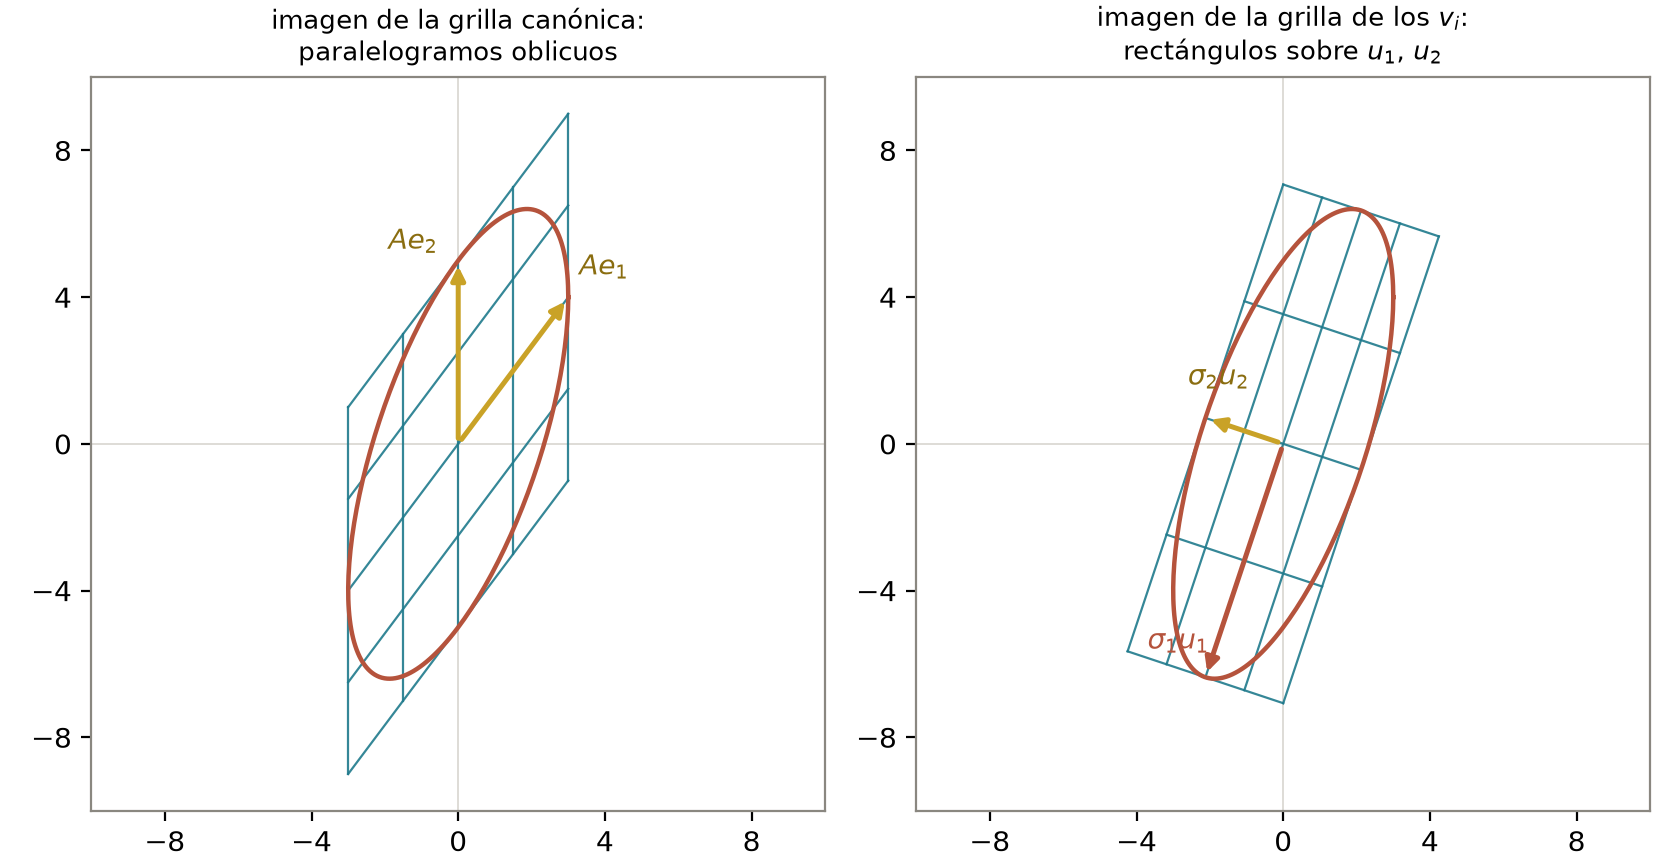
\includegraphics[width=.8\linewidth]{figuras/svd/svd_grilla.png}
\caption{Imagen por \(A=\left(\begin{smallmatrix}3&0\\4&5\end{smallmatrix}\right)\) de una
grilla cuadrada de lado \(2\), en la base canónica (izquierda) y en la base de los \(v_i\)
(derecha). En color óxido, la imagen de la circunferencia unidad, la misma en los dos
paneles. Generada con \texttt{apunte/scripts/cap07\_svd.py}.}
\label{fig:svd-grilla}
\end{figure}

\subsection{Simulaciones}

\unidadInteractiva{09_cambio_de_base_svd}{Cambio de base, SVD e inversas}{Verificá: con el caso «aplastante» comprobá que \(\sigma_2=0\) y que la elipse se reduce a un segmento.}

En la sección «Manipulación» de la unidad, cuatro deslizadores fijan las entradas de una
matriz de \(2\times2\) y la figura muestra la grilla deformada, la circunferencia unidad con
\(v_1\), \(v_2\) y la elipse imagen con \(\sigma_1u_1\), \(\sigma_2u_2\); la animación recorre
las tres etapas \(V^T\), \(\Sigma\), \(U\). Conviene probar los casos precargados (simétrica,
corte, aplastante con \(\sigma_2=0\), rotación pura) y observar cuándo la elipse se vuelve
circunferencia o segmento. Las cuentas del ejemplo~\ref{ej:svd-mano} se comprueban con el
script del capítulo o con tres líneas de NumPy:
\texttt{U, s, Vt = np.linalg.svd(A)}, \texttt{s**2} frente a
\texttt{np.linalg.eigvalsh(A.T @ A)} y \texttt{np.allclose(U @ np.diag(s) @ Vt, A)}.

\section{En profundidad}

\subsection{Plano ajustado a una nube de puntos}

Cuando las tres coordenadas de un punto
relevado tienen error, ajustar un plano \(z=ax+by+c\) por mínimos cuadrados ordinarios
privilegia indebidamente la \(z\). Lo natural es minimizar la suma de los cuadrados de las
distancias \emph{perpendiculares} al plano (mínimos cuadrados ortogonales). Si el plano tiene
normal unitaria \(w\) y pasa por el centroide \(\bar p\) de los puntos (para \(w\) fijo, la
mejor posición es la que pasa por el centroide, porque el promedio minimiza la suma de
cuadrados de los desvíos), la suma de distancias al cuadrado es
\[
  \sum_k\big((p_k-\bar p)\cdot w\big)^2=\|Xw\|^2 ,
\]
donde \(X\) es la matriz de \(N\times3\) cuyas filas son los \(p_k-\bar p\). Es la forma
cuadrática del capítulo, evaluada sobre la esfera unidad; por la
proposición~\ref{prop:svd-mide}, su mínimo es \(\sigma_3^2\) y se alcanza en \(w=v_3\), el
vector singular derecho del \emph{menor} valor singular: la dirección en que la nube es más
delgada.

\begin{ejemplo}[Plano por ocho puntos relevados]\label{ej:svd-plano}
El script genera \(N=8\) puntos sintéticos (semilla fija) cerca de un plano suavemente
inclinado, con un error de unos centímetros en la altura; en metros:
\begin{center}
\small
\begin{tabular}{crrr}
\toprule
\(k\) & \(x\) & \(y\) & \(z\)\\
\midrule
1 & 6{,}539 & 19{,}746 & 99{,}931\\
2 & 6{,}374 & 15{,}771 & 100{,}046\\
3 & 17{,}398 & 7{,}822 & 100{,}688\\
4 & 8{,}758 & 7{,}455 & 100{,}280\\
5 & 2{,}139 & 9{,}579 & 99{,}926\\
6 & 4{,}827 & 5{,}143 & 100{,}146\\
7 & 3{,}695 & 3{,}877 & 100{,}058\\
8 & 16{,}277 & 8{,}460 & 100{,}655\\
\bottomrule
\end{tabular}
\end{center}
El centroide es \(\bar p\approx(8{,}251;\ 9{,}732;\ 100{,}216)\). La SVD de la matriz
centrada \(X\) (\(8\times3\)) da \(\sigma_1\approx15{,}233\), \(\sigma_2\approx13{,}992\) y
\(\sigma_3\approx0{,}0607\): dos direcciones en las que la nube se extiende decenas de metros
y una en la que casi no tiene espesor. La normal es
\[
  v_3\approx(-0{,}0497;\ 0{,}0173;\ 0{,}9986),
\]
casi vertical: el plano está inclinado unos \(3{,}01^\circ\). El plano ajustado es
\((p-\bar p)\cdot v_3=0\). Las distancias con signo de los puntos al plano van de
\(-0{,}033\) m a \(0{,}027\) m, y la distancia cuadrática media es
\[
  \text{RMS}=\sqrt{\tfrac18\textstyle\sum_k d_k^2}=\frac{\sigma_3}{\sqrt8}\approx0{,}021\text{ m}.
\]
\end{ejemplo}

\subsection{Aplicación topográfica: la elipse de error de un punto GNSS}

Volvemos a la nube de la figura~\ref{fig:svd-nube}. Sea \(X\) la matriz de \(N\times2\) de
las posiciones centradas: cada fila es un desvío (este, norte) respecto del promedio. La
matriz de covarianza es
\[
  C=\frac1{N-1}X^TX .
\]
Es de la forma \(A^TA\) con \(A=X/\sqrt{N-1}\), así que todo lo anterior se aplica: si
\(X=U\Sigma V^T\), entonces \(C=V\,\frac{\Sigma^T\Sigma}{N-1}\,V^T\), de modo que los
autovectores de \(C\) son los vectores singulares derechos \(v_i\) de \(X\) y sus autovalores
son \(\lambda_i=\sigma_i^2/(N-1)\). La \emph{elipse de error} de un desvío es la curva de
nivel \(x^TC^{-1}x=1\); en la base de los \(v_i\) se escribe
\(y_1^2/\lambda_1+y_2^2/\lambda_2=1\), de modo que sus semiejes miden
\[
  \sqrt{\lambda_i}=\frac{\sigma_i}{\sqrt{N-1}}
\]
en las direcciones \(v_i\). La SVD de la matriz de datos da la elipse sin formar \(C\).

\paragraph{La elipse del \texorpdfstring{\(95\)\,\%}{95 \%}.} Las curvas de nivel
\(x^TC^{-1}x=k^2\) son la misma elipse escalada por \(k\). Si los errores siguen una
distribución normal bivariada, \(x^TC^{-1}x=y_1^2/\lambda_1+y_2^2/\lambda_2\) es la suma de
los cuadrados de dos variables normales estándar independientes, es decir, tiene
distribución \(\chi^2\) con dos grados de libertad, cuya función de distribución es
\(P(\chi^2_2\le t)=1-e^{-t/2}\). Pedir probabilidad \(0{,}95\) da
\(t=-2\ln0{,}05\approx5{,}991\), el percentil \(\chi^2_{2;\,0{,}95}\), y el factor de escala
es \(k=\sqrt{5{,}991}\approx2{,}448\). (Con \(k=1\), la elipse de un desvío, la probabilidad
es sólo \(1-e^{-1/2}\approx39\)\,\%.)

\begin{ejemplo}[Elipse de error de una nube GNSS sintética]\label{ej:svd-elipse-error}
Para las \(N=200\) posiciones de la figura~\ref{fig:svd-nube}, la SVD de la matriz centrada
\(X\) (\(200\times2\)) da \(\sigma_1\approx21{,}437\) y \(\sigma_2\approx9{,}087\), con
\(v_1\approx(0{,}859;\ 0{,}512)\) y \(v_2\approx(0{,}512;\ -0{,}859)\). Dividiendo por
\(\sqrt{199}\approx14{,}107\) se obtienen los semiejes de un desvío,
\(1{,}520\) m y \(0{,}644\) m. Por el otro camino,
\[
  C\approx\begin{pmatrix}1{,}813&0{,}833\\0{,}833&0{,}911\end{pmatrix}\ \text{m}^2,
  \qquad \lambda_1\approx2{,}309,\quad \lambda_2\approx0{,}415,
\]
y \(\sqrt{\lambda_1}\approx1{,}520\), \(\sqrt{\lambda_2}\approx0{,}644\): los mismos números.
El eje mayor \(v_1\) forma \(30{,}8^\circ\) con el este en sentido antihorario, es decir,
está orientado \(90^\circ-30{,}8^\circ=59{,}2^\circ\) respecto del norte, medido en sentido
horario como un acimut (sección~\ref{sec:acimut-campo}). Multiplicando por \(2{,}448\):
\emph{el \(95\)\,\% de las posiciones cae dentro de una elipse de semiejes \(3{,}72\) m y
\(1{,}58\) m, con el eje mayor orientado \(59{,}2^\circ\) respecto del norte}. En la nube
sintética caen adentro \(190\) de las \(200\) posiciones (\(95\)\,\%). Lectura topográfica:
la posición está determinada unas dos veces y media mejor en la dirección \(v_2\)
(acimut \(149{,}2^\circ\)) que en la \(v_1\).
\end{ejemplo}

\subsection{Otras lecturas de la misma elipse}

\paragraph{La elipse de distorsión de Tissot.} Una proyección cartográfica es, punto a punto,
aproximadamente lineal: su jacobiano lleva un desplazamiento infinitesimal del terreno a uno
del mapa. La imagen de una circunferencia infinitesimal es entonces una elipse, la
\emph{indicatriz de Tissot}, cuyos semiejes son los valores singulares del jacobiano (las
escalas máxima y mínima en ese punto) y cuyos ejes son las direcciones singulares de
salida. Una proyección es conforme cuando en cada punto \(\sigma_1=\sigma_2\) y la elipse es
una circunferencia; el desarrollo está en el complemento~\ref{cap:conformes}.

\paragraph{Aplicación al terreno.} Un modelo digital de elevación es una matriz de alturas, y
su SVD lo separa en relieves ordenados por importancia a partir de los cuales se trazan curvas
de nivel más o menos detalladas: ese desarrollo es el complemento~\ref{cap:dem}.

\subsection{Existencia de la SVD}

La demostración usa un resultado de álgebra lineal que no probamos en este apunte.

\begin{resultado}[Teorema espectral (resultado usado)]
Si \(M\) es una matriz real simétrica de \(n\times n\), sus autovalores son reales y existe
una base ortonormal de \(\R^n\) formada por autovectores de \(M\).
\end{resultado}

En el capítulo~\ref{cap:autovectores} los autovalores aparecen como factores de estiramiento
de las direcciones invariantes; el teorema espectral agrega que, para matrices simétricas,
esas direcciones existen siempre y pueden elegirse perpendiculares.

\begin{teorema}[Existencia de la SVD]\label{teo:svd-existencia}
Toda matriz real \(A\) de \(m\times n\) admite una descomposición en valores singulares
\(A=U\Sigma V^T\). Los valores singulares son las raíces cuadradas de los autovalores de
\(A^TA\): \(\sigma_i^2=\lambda_i(A^TA)\).
\end{teorema}

\begin{demostracion}
\emph{\(A^TA\) es simétrica y semidefinida positiva.} \((A^TA)^T=A^T(A^T)^T=A^TA\), y para
todo \(x\), \(x^TA^TAx=\|Ax\|^2\ge0\).

\emph{Base de la entrada.} Por el teorema espectral hay una base ortonormal
\(v_1,\dots,v_n\) de autovectores de \(A^TA\), con autovalores reales que ordenamos
\(\lambda_1\ge\dots\ge\lambda_n\). Son no negativos:
\(\lambda_i=\lambda_i\|v_i\|^2=v_i^TA^TAv_i=\|Av_i\|^2\ge0\). Definimos
\(\sigma_i=\sqrt{\lambda_i}=\|Av_i\|\) y llamamos \(r\) a la cantidad de \(\sigma_i>0\).

\emph{Base de la salida.} Para \(i\le r\) sea \(u_i=Av_i/\sigma_i\). Son ortonormales:
\[
  u_i\cdot u_j=\frac{v_i^TA^TAv_j}{\sigma_i\sigma_j}=\frac{\lambda_j\,v_i\cdot v_j}{\sigma_i\sigma_j},
\]
que vale \(1\) si \(i=j\) y \(0\) si \(i\neq j\). Si \(r<m\), completamos
\(u_1,\dots,u_r\) con vectores \(u_{r+1},\dots,u_m\) hasta una base ortonormal de \(\R^m\)
(por ejemplo, con Gram--Schmidt).

\emph{La factorización.} Para \(i\le r\), \(Av_i=\sigma_iu_i\) por definición; para
\(i>r\), \(\|Av_i\|=\sigma_i=0\), de modo que \(Av_i=0=\sigma_iu_i\). Con
\(V=[v_1\cdots v_n]\), \(U=[u_1\cdots u_m]\) y \(\Sigma\) de \(m\times n\) con
\(\sigma_1,\sigma_2,\dots\) en la diagonal, esas igualdades dicen \(AV=U\Sigma\). Como \(V\)
es ortogonal, \(V^{-1}=V^T\) y \(A=U\Sigma V^T\). Finalmente, \(A^TA=V\Sigma^T\Sigma V^T\)
muestra que los \(\sigma_i^2\) son los autovalores de \(A^TA\) en cualquier SVD.
\end{demostracion}

\paragraph{Por qué no aparecen números complejos.} Diagonalizar \(A\) puede fallar de dos
maneras: \(A\) puede no tener suficientes autovectores (un corte) o tener autovalores
complejos. La SVD no pregunta por los autovalores de \(A\) sino por los de \(A^TA\), que es
simétrica: sus autovalores son reales y no negativos, y sus autovectores pueden elegirse
perpendiculares. El ejemplo mínimo es la rotación de \(90^\circ\),
\[
  R=\begin{pmatrix}0&-1\\1&0\end{pmatrix},\qquad \det(R-\lambda I)=\lambda^2+1 ,
\]
cuyos autovalores son \(\pm i\): ninguna recta real queda fija. Pero \(R^TR=I\), los dos
valores singulares valen \(1\) y una SVD es simplemente \(R=R\cdot I\cdot I^T\) (\(U=R\),
\(\Sigma=I\), \(V=I\)). La circunferencia va a parar a sí misma; la curva \(\|Rx\|=1\) es la
circunferencia unidad. La rotación no estira nada, sólo gira, y la SVD lo dice sin salir de
los reales.

\subsection{Alcance de la lectura}

\begin{atencion}[Sólo para formas cuadráticas]
La SVD describe la forma \emph{exacta} de las curvas de nivel sólo cuando la función es
cuadrática, \(Q(x)=\|Ax\|^2\) (o una forma cuadrática con matriz semidefinida positiva).
Para una función general \(f\) describe únicamente la \emph{aproximación de segundo orden}
alrededor de un punto: si en \(x_0\) el gradiente se anula, cerca de \(x_0\) vale
\(f(x_0+h)\approx f(x_0)+\tfrac12h^THh\), con \(H\) la hessiana
(capítulo~\ref{cap:derivada}), y si \(H\) es definida positiva las curvas de nivel cercanas
se parecen a las elipses de esa forma cuadrática. Lejos de \(x_0\) las curvas pueden tener
cualquier forma, y donde el gradiente no se anula la aproximación dominante es la lineal:
las curvas se parecen localmente a rectas paralelas, como las de una forma lineal.
\end{atencion}

\paragraph{Lo que viene.} La SVD es un cambio de base, pero con una particularidad: usa
\emph{bases distintas} en la entrada (\(V\)) y en la salida (\(U\)), de modo que \(\Sigma\) no
es «\(A\) en otra base» en el sentido de la diagonalización y no sirve para calcular
potencias. Esa comparación es parte del capítulo~\ref{cap:cambio-base}. Y como cada etapa de
\(U\Sigma V^T\) se deshace por separado, una matriz cuadrada con todos los \(\sigma_i>0\)
tiene inversa \(A^{-1}=V\Sigma^{-1}U^T\); qué hacer cuando algún \(\sigma_i\) es cero o la
matriz es rectangular es el tema del capítulo~\ref{cap:inversas}.

\section{Ejercicios propuestos}

\begin{ejercicio}\label{ex:svd-corte}
Hallar la SVD de \(B=\begin{pmatrix}1&2\\0&1\end{pmatrix}\) y describir la curva de nivel
\(\|Bx\|=1\): direcciones de los ejes y largos de los semiejes. Verificar que
\(\sigma_1\sigma_2=|\det B|\).
\end{ejercicio}
\solucion{\(B^TB=\left(\begin{smallmatrix}1&2\\2&5\end{smallmatrix}\right)\), con
\(\lambda^2-6\lambda+1=0\), \(\lambda=3\pm2\sqrt2\approx5{,}828;\ 0{,}172\). Valores
singulares \(\sigma_1=1+\sqrt2\approx2{,}414\) y \(\sigma_2=\sqrt2-1\approx0{,}414\), con
\(\sigma_1\sigma_2=1=\det B\). Numpy da \(v_1\approx(0{,}383;\ 0{,}924)\) (a \(67{,}5^\circ\)
del eje \(x_1\)), \(v_2\approx(-0{,}924;\ 0{,}383)\), \(u_1\approx(0{,}924;\ 0{,}383)\),
\(u_2\approx(-0{,}383;\ 0{,}924)\). La curva \(\|Bx\|=1\) es una elipse de semieje corto
\(1/\sigma_1\approx0{,}414\) sobre \(v_1\) y semieje largo \(1/\sigma_2\approx2{,}414\)
sobre \(v_2\): muy alargada, aunque \(B\) conserva el área.}

\begin{ejercicio}\label{ex:svd-sigma-cero}
Sea \(D=\begin{pmatrix}1&2\\2&4\end{pmatrix}\). Mostrar que \(\sigma_2=0\), describir las
curvas de nivel de \(\|Dx\|\) y la imagen de la circunferencia unidad.
\end{ejercicio}
\solucion{\(D\) tiene rango \(1\): \(\sigma_1=5\), \(\sigma_2=0\), con
\(v_1=-(1,2)/\sqrt5\), \(v_2=(-2,1)/\sqrt5\) (signos de numpy) y \(u_1=-(1,2)/\sqrt5\).
Como \(\|Dx\|=5\,|v_1\cdot x|\), la curva \(\|Dx\|=1\) es el par de rectas paralelas
\(v_1\cdot x=\pm\tfrac15\), perpendiculares a \(v_1\) y a distancia \(1/\sigma_1=0{,}2\) del
origen: la elipse degeneró en una banda de semieje infinito sobre \(v_2\), el núcleo. La
circunferencia unidad va a parar al segmento de extremos \(\pm5u_1=\pm(\sqrt5,\,2\sqrt5)\),
recorrido dos veces.}

\begin{ejercicio}\label{ex:svd-estacion}
Una estación total entrega para un punto la matriz de covarianza (coordenadas este, norte)
\[
  C=\begin{pmatrix}13{,}6&4{,}8\\4{,}8&6{,}4\end{pmatrix}\ \text{mm}^2 .
\]
Hallar los semiejes de la elipse de error y la orientación del eje mayor (ángulo desde el
este y acimut). ¿En qué dirección está mejor determinada la posición?
\end{ejercicio}
\solucion{\(\det(C-\lambda I)=\lambda^2-20\lambda+64=0\) da \(\lambda_1=16\) y
\(\lambda_2=4\); semiejes \(4\) mm y \(2\) mm. El eje mayor tiene dirección \((2,1)/\sqrt5\)
(numpy la da con el signo opuesto, la misma recta), a \(26{,}57^\circ\) del este, acimut
\(63{,}43^\circ\). La posición está determinada el doble de bien en la dirección
perpendicular, \((-1,2)/\sqrt5\), de acimut \(333{,}43^\circ\). La correlación entre los
errores en este y norte es \(4{,}8/\sqrt{13{,}6\cdot6{,}4}\approx0{,}51\).}

\begin{ejercicio}\label{ex:svd-desdeformar}
Para \(A=\begin{pmatrix}3&0\\4&5\end{pmatrix}\) se conoce la SVD del
ejemplo~\ref{ej:svd-mano}: \(U=\frac1{\sqrt{10}}\left(\begin{smallmatrix}-1&-3\\-3&1\end{smallmatrix}\right)\),
\(\Sigma=\operatorname{diag}(3\sqrt5,\sqrt5)\),
\(V=\frac1{\sqrt2}\left(\begin{smallmatrix}-1&-1\\-1&1\end{smallmatrix}\right)\).
(a) Hallar una matriz que lleve la elipse imagen de la circunferencia unidad de vuelta a la
circunferencia unidad. (b) Hallar la que, además, devuelve cada punto de la elipse al punto
de la circunferencia del que salió. ¿Son la misma?
\end{ejercicio}
\solucion{(a) Basta deshacer los dos últimos movimientos: \(U^T\) lleva los ejes de la
elipse sobre los ejes coordenados y \(\Sigma^{-1}\) los encoge a largo \(1\). Así
\(\Sigma^{-1}U^T\approx\left(\begin{smallmatrix}-0{,}047&-0{,}141\\-0{,}424&0{,}141\end{smallmatrix}\right)\)
lleva la elipse sobre la circunferencia; por ejemplo, manda \(\sigma_1u_1\) a \((1,0)\). Cualquier
matriz ortogonal aplicada después también sirve, de modo que la respuesta no es única.
(b) Hay que deshacer además el primer giro: \(V\Sigma^{-1}U^T=A^{-1}
=\frac1{15}\left(\begin{smallmatrix}5&0\\-4&3\end{smallmatrix}\right)
\approx\left(\begin{smallmatrix}0{,}333&0\\-0{,}267&0{,}2\end{smallmatrix}\right)\),
que manda \(\sigma_1u_1\) de vuelta a \(v_1\approx(-0{,}707;\ -0{,}707)\). No son la misma:
difieren en el factor ortogonal \(V\), que gira la circunferencia sobre sí misma.}

\paragraph{Bibliografía del capítulo.} La presentación de la SVD a partir de \(A^TA\) y del
teorema espectral, con la interpretación de los cuatro subespacios, sigue el enfoque de
Strang, \emph{Álgebra lineal y sus aplicaciones}. Las formas cuadráticas, su reducción a
ejes principales y el ajuste por mínimos cuadrados están tratados en Noble y Daniel,
\emph{Álgebra lineal aplicada}, y en Goloviná, \emph{Álgebra lineal y algunas de sus
aplicaciones}.
